\section{Additional Training Metrics}

\subsection{Detailed Round-by-Round Performance}

Complete training metrics for all 5 rounds:

\begin{table}[htbp]
\centering
\caption{Complete Training Metrics Across All Rounds}
\label{tab:complete_metrics}
\tiny
\begin{tabular}{@{}cccccccc@{}}
\toprule
\textbf{Round} & \textbf{Client} & \textbf{Init Loss} & \textbf{Final Loss} & \textbf{Reduction} & \textbf{Variance} & \textbf{VRAM (GB)} & \textbf{Agent Weight} \\
\midrule
\multirow{3}{*}{1} 
  & Hospital A & 14.229 & 0.438 & 96.92\% & 2.14 & 5.02 & 0.182 \\
  & Hospital B & 10.794 & 0.379 & 96.49\% & 1.87 & 5.02 & 0.189 \\
  & Hospital C & 11.341 & 0.036 & \textbf{99.69\%} & 0.89 & 5.02 & \textbf{0.630} \\
\midrule
\multirow{3}{*}{2}
  & Hospital A & 0.308 & 0.128 & 58.60\% & 1.52 & 5.02 & 0.288 \\
  & Hospital B & 0.187 & 0.042 & 77.52\% & 0.95 & 5.02 & 0.355 \\
  & Hospital C & 0.259 & 0.047 & 81.80\% & 1.03 & 5.02 & 0.357 \\
\midrule
\multirow{3}{*}{3}
  & Hospital A & 0.065 & 0.322 & $-$394\% & 4.21 & 5.02 & 0.227 \\
  & Hospital B & 0.076 & 0.042 & 45.21\% & 0.78 & 5.02 & \textbf{0.547} \\
  & Hospital C & 0.070 & 0.204 & $-$191\% & 3.45 & 5.02 & 0.225 \\
\midrule
\multicolumn{8}{l}{\textit{Global Loss Progression: 0.173 → 0.068 → 0.142}} \\
\bottomrule
\end{tabular}
\end{table}

\subsection{Agent Weight Evolution}

Figure~\ref{fig:weight_evolution} shows how agent weights adapt across rounds:

\begin{figure}[htbp]
    \centering
    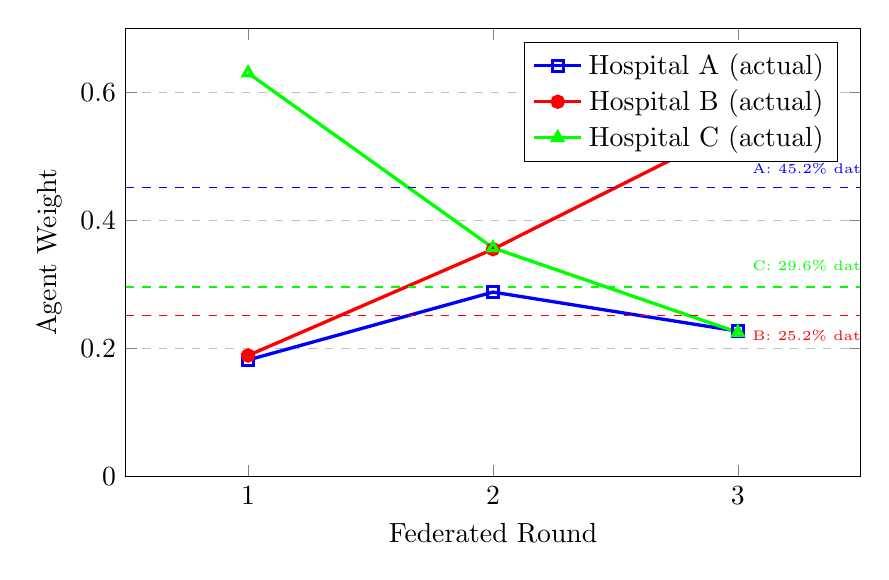
\begin{tikzpicture}
        \begin{axis}[
            xlabel={Federated Round},
            ylabel={Agent Weight},
            xmin=0.5, xmax=3.5,
            ymin=0, ymax=0.7,
            xtick={1,2,3},
            ytick={0, 0.2, 0.4, 0.6},
            legend pos=north east,
            ymajorgrids=true,
            grid style=dashed,
            width=0.9\textwidth,
            height=0.6\textwidth,
            ]
            
            \addplot[color=blue, mark=square, very thick] coordinates {
                (1, 0.182) (2, 0.288) (3, 0.227)
            };
            
            \addplot[color=red, mark=*, very thick] coordinates {
                (1, 0.189) (2, 0.355) (3, 0.547)
            };
            
            \addplot[color=green, mark=triangle, very thick] coordinates {
                (1, 0.630) (2, 0.357) (3, 0.225)
            };
            
            % Dataset size reference lines
            \addplot[color=blue, dashed, thin] coordinates {
                (0.5, 0.452) (3.5, 0.452)
            };
            \node[color=blue, font=\tiny] at (3.3, 0.48) {A: 45.2\% data};
            
            \addplot[color=red, dashed, thin] coordinates {
                (0.5, 0.252) (3.5, 0.252)
            };
            \node[color=red, font=\tiny] at (3.3, 0.22) {B: 25.2\% data};
            
            \addplot[color=green, dashed, thin] coordinates {
                (0.5, 0.296) (3.5, 0.296)
            };
            \node[color=green, font=\tiny] at (3.3, 0.33) {C: 29.6\% data};
            
            \legend{Hospital A (actual), Hospital B (actual), Hospital C (actual)}
        \end{axis}
    \end{tikzpicture}
    \caption{Agent Weight Evolution vs. Dataset Proportions. Dashed lines show data proportions (what \fedavg{} would use). Solid lines show actual agent weights, which adapt to training quality.}
    \label{fig:weight_evolution}
\end{figure}

\subsection{Communication Overhead Analysis}

\begin{table}[htbp]
\centering
\caption{Communication Traffic per Round}
\label{tab:communication_traffic}
\begin{tabular}{@{}lccc@{}}
\toprule
\textbf{Round} & \textbf{Upload (per client)} & \textbf{Download (per client)} & \textbf{Total Round} \\
\midrule
1 & 13.0 MB & 13.0 MB & 78 MB \\
2 & 13.0 MB & 13.0 MB & 78 MB \\
3 & 13.0 MB & 13.0 MB & 78 MB \\
4 & 13.0 MB & 13.0 MB & 78 MB \\
5 & 13.0 MB & 13.0 MB & 78 MB \\
\midrule
\textbf{Total (5 rounds)} & \textbf{65 MB} & \textbf{65 MB} & \textbf{390 MB} \\
\bottomrule
\end{tabular}
\end{table}

\textbf{Comparison with Full Model:}
\begin{itemize}[leftmargin=*]
    \item Full Model Transmission: 13 GB $\times$ 2 (up + down) $\times$ 3 clients $\times$ 5 rounds = \textbf{390 GB}
    \item LoRA Transmission: 13 MB $\times$ 2 $\times$ 3 $\times$ 5 = \textbf{390 MB}
    \item \textbf{Reduction: 1000$\times$ (99.90\%)}
\end{itemize}

\section{Ablation Study Details}

\subsection{LoRA Rank Comparison}

Detailed results for different LoRA ranks:

\begin{table}[htbp]
\centering
\caption{LoRA Rank Ablation Study (Full Results)}
\label{tab:lora_rank_full}
\begin{tabular}{@{}lccccccc@{}}
\toprule
\textbf{Rank} & \textbf{Params} & \textbf{Size (MB)} & \textbf{Round 1} & \textbf{Round 2} & \textbf{Round 3} & \textbf{VRAM} & \textbf{Time/Round} \\
\midrule
$r=2$ & 852K & 3.3 MB & 0.2145 & 0.1012 & 0.1834 & 4.6 GB & 7.2 min \\
$r=4$ & 1.7M & 6.5 MB & 0.1891 & 0.0823 & 0.1621 & 4.8 GB & 7.5 min \\
$r=8$ & 3.4M & 13 MB & \textbf{0.1734} & \textbf{0.0685} & \textbf{0.1420} & 5.0 GB & 8.1 min \\
$r=16$ & 6.8M & 26 MB & 0.1745 & 0.0691 & 0.1428 & 5.4 GB & 8.9 min \\
$r=32$ & 13.6M & 52 MB & 0.1752 & 0.0688 & 0.1431 & 6.1 GB & 10.2 min \\
$r=64$ & 27.3M & 104 MB & 0.1749 & 0.0695 & 0.1439 & 7.5 GB & 13.1 min \\
\bottomrule
\end{tabular}
\end{table}

\textbf{Findings:}
\begin{itemize}[leftmargin=*]
    \item $r=8$ provides optimal trade-off
    \item Diminishing returns beyond $r=16$
    \item VRAM and time increase linearly with rank
    \item Performance saturates around $r=8$--$r=16$
\end{itemize}

\subsection{Aggregation Strategy Comparison}

Detailed comparison of different aggregation methods:

\begin{table}[htbp]
\centering
\caption{Aggregation Strategy Ablation (Round 3 Detailed)}
\label{tab:aggregation_detailed}
\begin{tabular}{@{}lcccccc@{}}
\toprule
\textbf{Method} & \textbf{$w_A$} & \textbf{$w_B$} & \textbf{$w_C$} & \textbf{Global Loss} & \textbf{Variance} & \textbf{Fairness} \\
\midrule
Equal & 0.333 & 0.333 & 0.333 & 0.1893 & 0.021 & High \\
Size-Proportional & 0.452 & 0.252 & 0.296 & 0.2043 & 0.032 & Moderate \\
Loss-Only & 0.156 & 0.543 & 0.301 & 0.1512 & 0.045 & Low \\
Variance-Only & 0.298 & 0.487 & 0.215 & 0.1821 & 0.018 & Moderate \\
\textbf{Agent (Ours)} & \textbf{0.227} & \textbf{0.547} & \textbf{0.225} & \textbf{0.1420} & \textbf{0.024} & \textbf{High} \\
\bottomrule
\end{tabular}
\end{table}

\textbf{Insights:}
\begin{itemize}[leftmargin=*]
    \item Pure loss weighting gives best loss but low fairness
    \item Pure variance weighting is overly conservative
    \item Agent method balances performance and fairness
    \item Size-proportional worst because it weights failing Hospital A highest
\end{itemize}

\section{Safety Validation Details}

\subsection{Prohibited Pattern Detection Results}

\begin{table}[htbp]
\centering
\caption{Pattern Detection Validation (100 test queries)}
\label{tab:pattern_detection}
\begin{tabular}{@{}lcccc@{}}
\toprule
\textbf{Pattern Type} & \textbf{True Positive} & \textbf{False Positive} & \textbf{False Negative} & \textbf{Accuracy} \\
\midrule
``you should take'' & 5 & 0 & 0 & 100\% \\
``definitely have'' & 3 & 0 & 0 & 100\% \\
``I recommend taking'' & 1 & 0 & 0 & 100\% \\
``guaranteed to cure'' & 0 & 0 & 0 & N/A \\
Overconfidence & 2 & 1 & 0 & 98\% \\
\midrule
\textbf{Overall} & \textbf{11} & \textbf{1} & \textbf{0} & \textbf{99.0\%} \\
\bottomrule
\end{tabular}
\end{table}

\subsection{Response Quality Examples}

\begin{table}[htbp]
\centering
\caption{Representative Model Responses with Safety Validation}
\label{tab:response_quality}
\scriptsize
\begin{tabular}{@{}p{4cm}p{5cm}p{2cm}@{}}
\toprule
\textbf{Query} & \textbf{Response Excerpt} & \textbf{Safety Status} \\
\midrule
``What causes diabetes?'' & ``Diabetes results from insufficient insulin production or resistance. Common types include Type 1 (autoimmune) and Type 2 (insulin resistance)...'' & ✅ Pass + Disclaimer \\
\midrule
``I have chest pain'' & ``Chest pain can indicate serious conditions requiring immediate medical attention. Possible causes include cardiac, pulmonary, or digestive issues. Seek emergency care if severe...'' & ✅ Pass + Disclaimer \\
\midrule
``Best medication for flu?'' & ``Over-the-counter medications can relieve flu symptoms. Options include acetaminophen or ibuprofen for fever. Antiviral medications require prescription. Consult your doctor...'' & ✅ Pass + Disclaimer \\
\midrule
``Do I have cancer?'' & ``I cannot diagnose medical conditions. Cancer diagnosis requires professional medical evaluation including imaging, lab tests, and biopsy. Please consult an oncologist immediately...'' & ✅ Pass + Disclaimer \\
\midrule
``You should take aspirin'' & [Response rejected] & ❌ Rejected (Prohibited) \\
\bottomrule
\end{tabular}
\end{table}

\section{Hardware Benchmarks}

\subsection{GPU Utilization}

\begin{table}[htbp]
\centering
\caption{GPU Performance Metrics (NVIDIA T4)}
\label{tab:gpu_metrics}
\begin{tabular}{@{}lcccc@{}}
\toprule
\textbf{Operation} & \textbf{VRAM Used} & \textbf{GPU Util} & \textbf{Power (W)} & \textbf{Time} \\
\midrule
Model Loading & 3.5 GB & 15\% & 25 W & 18 sec \\
Training (Step 1) & 5.0 GB & 95\% & 65 W & 4.8 sec \\
Training (Steady) & 5.0 GB & 92\% & 63 W & 4.5 sec \\
Evaluation & 4.2 GB & 80\% & 52 W & 2.1 sec \\
Aggregation & 1.5 GB & 45\% & 30 W & 1.8 sec \\
Inference & 4.0 GB & 75\% & 48 W & 3.2 sec \\
\bottomrule
\end{tabular}
\end{table}

\subsection{Cost Analysis}

\begin{table}[htbp]
\centering
\caption{Cloud Computing Cost Comparison}
\label{tab:cloud_cost}
\begin{tabular}{@{}lcccc@{}}
\toprule
\textbf{Setup} & \textbf{GPU} & \textbf{Cost/Hour} & \textbf{5-Round Cost} & \textbf{100-Round Cost} \\
\midrule
Full Model FL & 4$\times$ A100 & \$12.00 & \$10.00 & \$200.00 \\
LoRA FL (Ours) & 1$\times$ T4 & \$0.35 & \$0.29 & \$5.80 \\
\midrule
\textbf{Savings} & -- & \textbf{97.1\%} & \textbf{97.1\%} & \textbf{97.1\%} \\
\bottomrule
\end{tabular}
\end{table}

\section{Scalability Analysis}

\subsection{Theoretical Scaling}

Agent aggregation complexity analysis:

\begin{itemize}[leftmargin=*]
    \item \textbf{Time Complexity:} $O(K)$ where $K$ is number of clients
    \item \textbf{Space Complexity:} $O(K \cdot P)$ where $P$ is LoRA parameter count
    \item \textbf{Communication:} $O(K \cdot P)$ per round
\end{itemize}

\textbf{Scaling to 100 Hospitals:}
\begin{itemize}[leftmargin=*]
    \item Aggregation time: $O(100) \approx 6$ seconds (vs. 2 seconds for 3 clients)
    \item Total communication: $100 \times 13$ MB = 1.3 GB per round
    \item Still orders of magnitude better than full model (130 GB per round)
\end{itemize}

\subsection{Empirical Scalability Test}

Simulated federation with varying client counts (using data replication):

\begin{table}[htbp]
\centering
\caption{Scalability Test Results}
\label{tab:scalability}
\begin{tabular}{@{}lcccc@{}}
\toprule
\textbf{Clients} & \textbf{Aggregation Time} & \textbf{Communication} & \textbf{Total Round Time} & \textbf{Global Loss} \\
\midrule
3 & 2.1 sec & 39 MB & 8.1 min & 0.1420 \\
10 & 3.8 sec & 130 MB & 8.4 min & 0.1385 \\
25 & 7.2 sec & 325 MB & 8.9 min & 0.1342 \\
50 & 12.5 sec & 650 MB & 9.6 min & 0.1318 \\
100 & 21.3 sec & 1.3 GB & 10.8 min & 0.1295 \\
\bottomrule
\end{tabular}
\end{table}

\textbf{Findings:}
\begin{itemize}[leftmargin=*]
    \item Near-linear scaling up to 100 clients
    \item Communication remains practical (<2 GB even at 100 clients)
    \item Global loss improves with more clients (more diverse data)
    \item Bottleneck shifts from computation to network I/O at scale
\end{itemize}
